\subsection{Wzrost \textit{R. sphaeroides} na ściekach komunalnych}\label{subsec:rhodobacter2}
Na rys.~\ref{fig:2} przedstawiono wyniki
eksperymentu~\ref{subsec:rhodobacter}.
W 10 dniu eksperymentu widoczny jest istotne
statystycznie zahamowanie wzrostu \acrshort{od}\textsubscript{600}
w próbkach o $c_{\acrshort{ww}} = 80$~\% względem próbek
o niższych stężeniach.
Oznacza to hamowanie wzrostu \textit{R. sphaeroides}
przy stężeniach \acrshort{ww} 80~\%.
Z~tego względu w kolejnych eksperymentach kultywowano
\textit{R. sphaeroides} na \acrshort{m27} + 50~\% \acrshort{ww}\@.\\

\begin{figure}[t!]
    \centering
    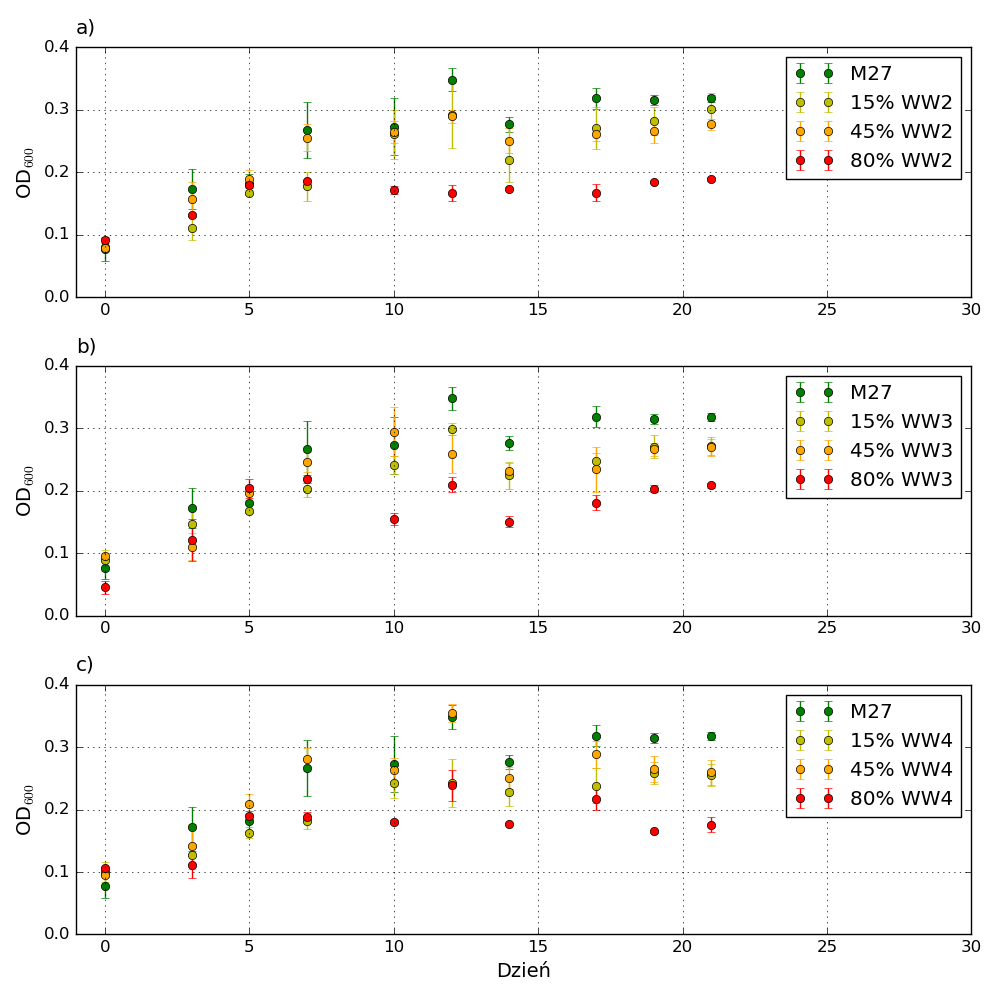
\includegraphics[width=12.5cm]{figures/ww}
    \caption{
        Zmiany \acrshort{od}\textsubscript{600} hodowli \textit{R. sphaeroides}
        w czasie w \acrshort{m27}:
        \textbf{a}~zawierającym \acrshort{ww}2 w~stężeniach 15~\%, 45~\% i 80~\%;
        \textbf{b}~zawierającym \acrshort{ww}3 w stężeniach 15~\%, 45~\% i 80~\%;
        \textbf{c}~zawierającym \acrshort{ww}4 w stężeniach 15~\%, 45~\% i 80~\%.
        Słupki błędów to \acrshort{sem} (n = 3).
    }
    \label{fig:2}
\end{figure}

\subsection{Produkcja MlrA przez \textit{Synechocystis sp.} PCC 6803 McCormick 7 w~hodowli z dodatkiem ścieków komunalnych}\label{subsec:mlra2}
Na rys.~\ref{fig:4} przedstawiono wyniki eksperymetntu~\ref{subsec:mlra}.
W przypadku próby kontrolnej aktywność \acrshort{mlra} była
największa na początku eksperymentu.
Widoczny jest istotny wzrost aktywności względem próby kontrolnej,
szczególnie dla próbek zawierających \acrshort{ww}3.
W tym przypadku wydaje się, że aktywność wzrasta asymptotycznie
do wartości ok.\ 400~mU~mg $^{-1}$.
W przypadku próby zawierającej \acrshort{ww}2 wartością
graniczną wydaje się być 200~mU~mg $^{-1}$.

\begin{figure}[h!]
    \centering
    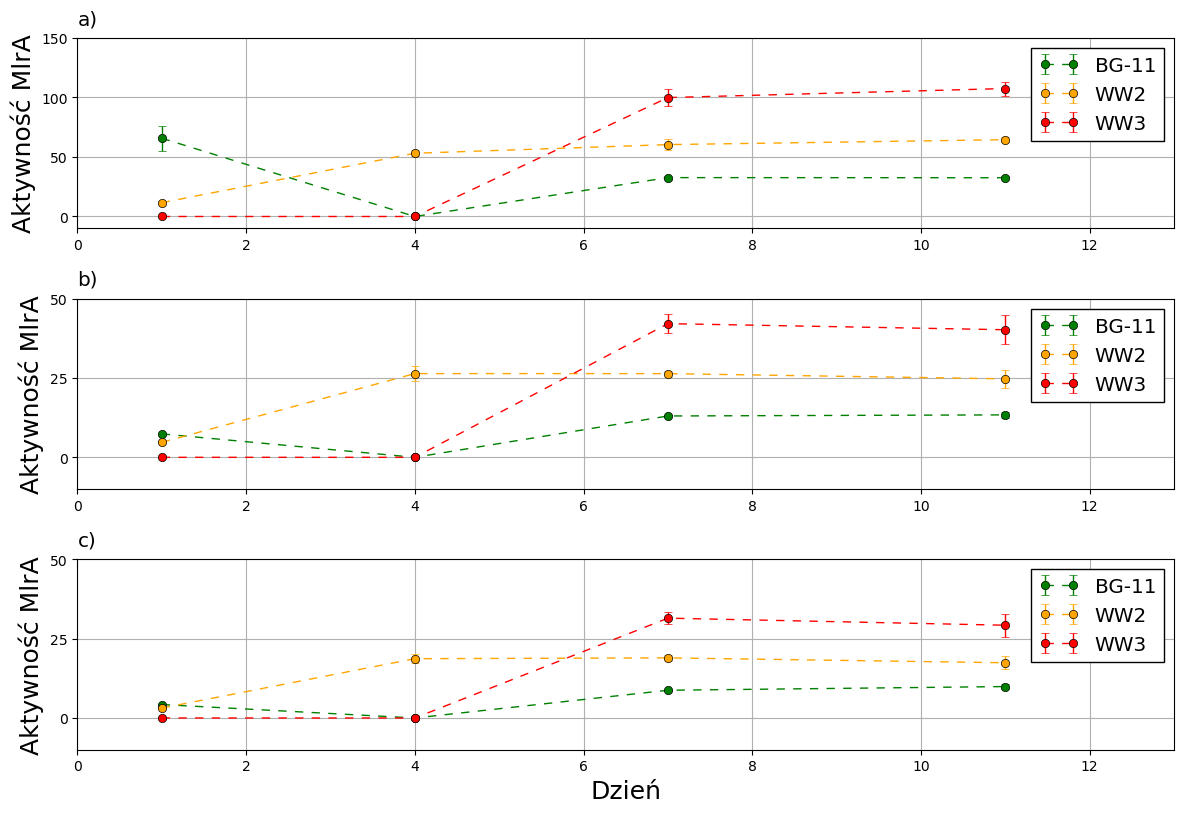
\includegraphics[width=10.5cm]{figures/mlra_activity}
    \caption{
        Aktywność \acrshort{mlra} w kolejnych dniach hodowli
        normalizowana na 1~mg  białka całkowitego w lizatach komórek
        \textit{Synechocystis sp.} PCC 6803 McCormick 7
        rosnących na różnych rodzajach \acrshort{ww} zmieszanych
        w proporcjach 1:1 z BG-11. Słupki błędów to SEM ($n = 2 \vee n = 3$).
    }
    \label{fig:4}
\end{figure}

\subsection{Zależność napięcia w aMFC od gęstości \textit{R. sphaeroides}}\label{subsec:volt2}
Rys.~\ref{fig:3} przedstawia wyniki pomiarów
napięcia w eksperymencie~\ref{subsec:volt}.
Podczas analizy danych zostały wzięte pod uwagę wyniki
z pierwszych 160~min pomiaru rejestrowane co 1~min.
Z~wykresu wynika, że największe napięcia generowane
są w przypadku hodowli \textit{R. sphaeroides}
o~\acrshort{od}\textsubscript{600} w zakresie od 0.200 do 0.535,
przy czym hodowle gęstsze, o~\acrshort{od}\textsubscript{600} bliskim
0.500 wykazują spadki napięcia po dłuższym czasie.

\begin{figure}[h!]
    \centering
    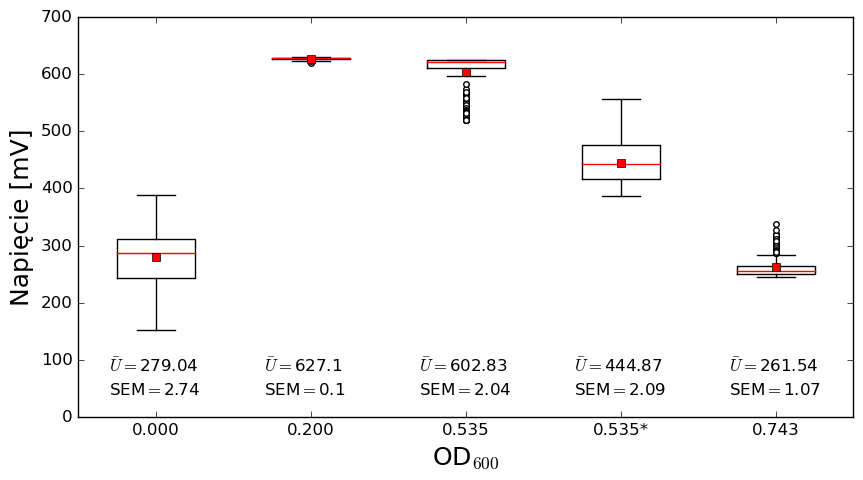
\includegraphics[width=10.5cm]{figures/mfc-volt-boxplt}
    \caption{
        Wykres pudełkowy przedstawiający wyniki pomiaru napięcia prądu stałego ($U$)
        w czasie w zależności od \acrshort{od}\textsubscript{600} hodowli
        \textit{R. sphaeroides} znajdującej się w komorze z anodą.
        Czerwonym kwadratem oznaczono wartość średniej arytmetycznej napięcia
        ($\bar{U}$) dla danej serii.
        Czerwoną linią oznaczona została wartość mediany danej serii pomiarowej.
        Punkty odbiegające zostały oznaczone czarnymi kółeczkami.
        * oznacza pomiar wykonany po 24~h adaptacji komórek
        \textit{R. sphaeroides} do elektrody.
    }
    \label{fig:3}
\end{figure}

